\documentclass{article}

\usepackage{subfig}
\usepackage{graphicx}

\usepackage{hyperref}
\usepackage{amsfonts}
\usepackage{cite}
\usepackage{amsmath,amsthm,amssymb}
\usepackage[noend]{algpseudocode}
\usepackage[margin=1.5in]{geometry}
\usepackage{algorithm}
\bibliographystyle{authordate1}
\usepackage[square, sort]{natbib}
\usepackage[utf8]{inputenc}
\usepackage{multicol}
\newcommand\inner[2]{\langle #1, #2 \rangle}
\newcommand*\Let[2]{\State #1 $\gets$ #2}
\algrenewcommand\algorithmicrequire{\textbf{Precondition:}}
\algrenewcommand\algorithmicensure{\textbf{Postcondition:}}
\newtheorem{theorem}{Theorem}[section]
\newtheorem{lemma}[theorem]{Lemma}
\newcommand*\conj[1]{\overline{#1}}
\newcommand*\bb[1]{\mathbb{#1}}
\newcommand*\cc[1]{\mathcal{#1}}
\newcommand*\wto{\rightharpoonup}
\newcommand*\Id{\text{Id}}
\newcommand*\im{\text{im}}
\DeclareMathOperator{\spn}{span}
\DeclareMathOperator{\dimens}{dim}
\newtheorem{innercustomgeneric}{\customgenericname}
\providecommand{\customgenericname}{}
\newcommand{\newcustomtheorem}[2]{%
  \newenvironment{#1}[1]
  {%
   \renewcommand\customgenericname{#2}%
   \renewcommand\theinnercustomgeneric{##1}%
   \innercustomgeneric
  }
  {\endinnercustomgeneric}
}

\newcustomtheorem{customthm}{Theorem}
\newcustomtheorem{customlemma}{Lemma}

\title{6.853 Final Project: Generalization and Equilibrium in Generative Adversarial Nets}
\author{Logan Engstrom and Kenny Gea}
\date{\today}

\begin{document}
\maketitle

\section{Literature Review}
\subsection{Introduction}
Generative Adversarial Networks (GANs) are a neural network framework introduced by \citet{Goodfellow2014} for estimating generative models from data. The framework consists of two models, a generator $G$ that captures the distribution of the data, and a discriminator $D$ that predicts the probability that a given sample is from the true data distribution or from the distribution estimated by $G$. Intuitively, $D$ is trained by minimizing the probability of making a mistake in classifying samples, and $G$ is trained by maximizing the probability that $D$ makes a mistake. The framework corresponds to a two player minimax game, so in the space of functions for $G$, $D$, there must exist a $(G,D)$ solution corresponding to a Nash Equilibrium. Since their inception, GANs have become the dominant method for fitting generative models to complex data \citep{Arora17} and have been applied to a variety of problems successfully, such as creating cryptographic protocols \citep{Abadi16} and aiding reinforcement learning \citep{FinnGL16}.

\subsection{Theoretical and Practical Limitations of GANs}
Despite the promise of GANs, fundamental problems in training and architecting GANs persist. Training GANs requires finding a Nash equilibrium of a non convex game parameterized in a high-dimensional, continuous space, a difficult problem \citep{Goodfellow17} \citep{Salimans2016}. In addition, in the traditional GAN setup we must find a pure Nash equilibrium \citep{Arora17}, which does not necessarily exist for general games. Generally GANs are trained using iterative gradient descent optimization techniques designed to find the minimum of a cost function – in particular, these optimization techniques are not designed to find the Nash equilibrium of a game \citep{Salimans2016}. As a result, sometimes when these algorithms are used for finding Nash equilibria they do not converge; one common problem is reaching a stable orbit, in which a modification to the discriminator's parameters that reduces the discriminator cost could in turn increase the generator’s cost. Then in the next round a modification to the generator’s parameters reduces the generator’s cost, but increases the discriminator cost, creating a circular feedback loop in which the algorithm never reaches equilibrium \citep{Salimans2016}. In general, training instability makes GANs often very hard to train \citep{DBLP:journals/corr/GulrajaniAADC17}.
\\
GANs have practical issues beyond the lack of theoretical guarantees and general training difficulties. Despite breakthroughs in speed and accuracy of generative models for images, larger scale images generated with GANs often lose finer texture details and have recurring artifacts \citep{DBLP:journals/corr/LedigTHCATTWS16} \citep{Salimans2016} \citep{DBLP:journals/corr/ShrivastavaPTSW16}. In addition to problems generating images, the application of GANs to discrete problems is limited due to the difficulty of backpropagation through discrete random variables, along with the general instability of the GAN training objective \citep{Che+al-2017-augmented}. 

\subsection{Recent GAN Improvements}
Experimentally driven GAN research has recently included applying traditional artificial neural networks architectures to GANs. One particularly successful such endeavor has been the application of deep convolutional layers to classical GAN problems such as image generation, such as with the DCGAN architecture \citep{DBLP:journals/corr/RadfordMC15}. Possibly the most active area of research has been in improving training for GANs, with much of recent work on GANs focussing on finding ways of stabilizing GAN training \citep{Salimans2016} \citep{DBLP:journals/corr/ArjovskyCB17} \citep{DBLP:conf/nips/NowozinCT16} \citep{DBLP:journals/corr/MetzPPS16}. \citet{DBLP:journals/corr/RadfordMC15} published guidelines on how to architect the generator and discriminator for more stable training. They provide specific recommendations based on experimental research, such the use of batch normalization in both networks and the deployment of LeakyReLU activations in the discriminator only. In addition, \citet{DBLP:journals/corr/HjelmJCCB17} provides a solution for more stable training for discrete generative problems using the GAN architecture. \citet{Salimans2016} provides another set of solutions for more stable GAN training. They introduce historical averaging of parameters in an attempt to compensate for the stable orbit problem, feature mapping to modify the loss function to fit on intermediate layer activations rather than the final layer activations, and a few other small architectural changes. \citet{Salimans2016} also introduced a now-popular evaluation metric for image based GANs based off of accuracy when classifying generated images with the Inception image classification network. One of the most important works in GAN research was \citet{DBLP:journals/corr/ArjovskyCB17}, which introduced a new training objective and architecture (the Wasserstein GAN) that empirically appears to lead to more stable training. Since the Wasserstein GAN was released, a variety of other papers building on the idea have emerged. One example is \citet{DBLP:journals/corr/GulrajaniAADC17}, which provides additional empirically researched methods for better GAN stability. In particular, \citep{Arora17} builds on several aspects of the Wasserstein GAN results. 

\subsection{Future GAN Work}
GANs are relatively new and are not fully understood at a theoretical level. Particularly, training GANs requires finding a Nash equilibrium for high dimensional, continuous, non-convex games, an area of active research that has applications outside of just GANs. Other theoretically oriented open problems in GANs include guaranteeing convergence for certain objectives and architectures, and proving that solutions exist at all for certain objectives and architectures \citep{Arora17}. In addition, GAN objectives cannot ensure that synthetic distributions resulting from generator functions have high diversity \citep{Arora17}. Other future GAN research will focus on discrete problems \citep{Che+al-2017-augmented}. Currently, both the generator and discriminator need to have their values be continuous. However, many interesting problems such as natural language processing have discrete inputs, severely limiting the application of GANs. The state of the art solution to transform the discrete space into a continuous space, which has mostly produced unsatisfactory results \citep{Che+al-2017-augmented}.

\section{Paper Implementation}
\subsection{Overview}
We implemented results from \cite{Arora17}. The paper's makes several contributions. First, the paper defines generalization; given a metric and two distributions, training generalizes if empirical distance, or the distance between the empirical distributions induced by the true distributions, approximates the distance between the true distributions. Note that when we train GANs, we are training the generator and discriminator off of empirical distributions (of the generator and of the generator's target distribution). The paper motivates the definition by showing that with high probability, for certain distributions, if the number of samples $m$ is not exponential in the dimensionality of the distribution then the Wasserstein distance:
\[
  d_W(\mu, \nu) = \sup\limits_{f : 1 \mbox{ Lipschitz} } \mathop{\bb{E}}\limits_{x \sim \mu}[f(x)] - \mathop{\bb{E}}\limits_{x \sim \nu} [f(x)]
\]
 and Jenson Shannon distance:
\[
  d_{JS}(\mu, \nu) = \frac{1}{2}(KL(\mu \| \frac{\mu+\nu}{2}) + KL(\nu \| \frac{\mu+\nu}{2}))
\]
do not generalize. The paper then introduces the ``Neural Network'' metric (where we have our class of discriminators defined as $\{D_v : v \in \cc{V}\}$, $\cc{V}$ as the space of parameters):
\[
  d_{NN}(\mu, \nu) = \max\limits_{v \in \cc{V}} \vert \mathop{\bb{E}}\limits_{x \sim \mu}[D_v(x)] - \mathop{\bb{E}}\limits_{x \sim \nu}[D_v(x)] \vert
\]
And shows that it does generalize (Theorem $3.3$). Next, in Section 4 of the paper, the authors show that an approximate pure equlibrium in the 2-player game exists for the Wasserstein training objective with a finite number of strategies. This result then motivates the paper's proposed protocol, MIX+GAN. The protocol for MIX+GAN is identical to a traditional GAN mechanism, except that the generator and discriminator functions are different - they are mixtures of traditional neural networks instead of a single network. The generator function $G$ in MIX-GAN is composed of $k$ neural network generators instead of just one. Each step, given a random input $h$, $h$ is run through each generator. Then one of the generators are chosen at random, with learned weights representing the probability that each generator is chosen. The generator selection mechanism is fully differentiable, as it is a two layer neural network. For the discriminator function, we take a (weighted, with learned weights) mixture of $k$ traditional neural network discriminators. If we have discriminator networks $D_{v_1},...,D_{v_k}$, then our overall discriminator function is, given a sample $x$ and weights $w_{v_i}$:
\[
  D(x) = \sum\limits_{i = 1}^k D_{v_i}(x) w_{v_i} \mbox{  } (\mbox{s.t.} \sum\limits_{i=1}^k w_{v_i} = 1)
\]
Note $D$ is also fully differentiable. The way the generator function and discriminator functions in MIX+GAN are defined make the payoffs for $D$ and $G$ identical to the payoffs for the mixtures of the component discriminators and generators. Note that large numbers of generators/discriminators are impractical, so the authors just choose a $k$ large as can fit on the GPU's memory (often the theoretically justified $k$ for an approximate Nash Equilibrium is much larger than can fit on current GPUs).

\subsection{Implementation Details}
We implemented MIX+GAN with ..........

Our implementation can be found at: \url{https://github.com/kennygea/6853-project}.

\subsection{Results}
The results are..........

\subsection{Discussion}
MIX+GAN provides an extension to traditional GANs. It is relatively easy to implement, and requires little hyperparameter tuning - important considering the general difficulties encountered when training GANs. MIX+GAN does not significantly advance the state of the art in terms of beating benchmarks or in terms of providing significantly higher quality qualitative results as compared to other leading GAN architectures, such as \citet{DBLP:journals/corr/HuangLPHB16}, \citet{Salimans2016}, and \citet{DBLP:journals/corr/OdenaOS16}. \citet{Arora17} also does provide the first proof that an approximate pure equilibrium exists with a certain distance metric (the Wasserstein metric). Importantly, however, the paper does not prove any guarantees about whether any given algorithm (such as backpropagation, in the paper's work) can actually find it. One of the problems in the paper is that the results are difficult to benchmark against other methods, as few quantitative measures are given and qualitatively the results shown are difficult to differentiate from the benchmarks presented in the paper (e.g., the MIX+DCGAN MNIST results don't look particularly different or improved from the original DCGAN MNIST results).


\bibliography{references.bib}
\newpage
\section*{Figures}
% \begin{figure}
%   \centering
%   \begin{subfigure}[b]
    
%     \caption{MIX+DCGAN with 5 Generators and 5 Discriminators on CelebA Dataset}
%     \label{fig:CelebA_T=5_Sample}
%   \end{subfigure}
%   \begin{subfigure}[b]
%     \caption{DCGAN on CelebA Dataset}
%     \label{fig:CelebA_T=1_Sample}
%   \end{subfigure}
%   \caption{MIX vs Non-MIX Samples from Training on CelebA}
% \end{figure}
\begin{figure}[!htb]%
  \centering
  \subfloat[][]{%
    \label{fig:fig1-a}%
    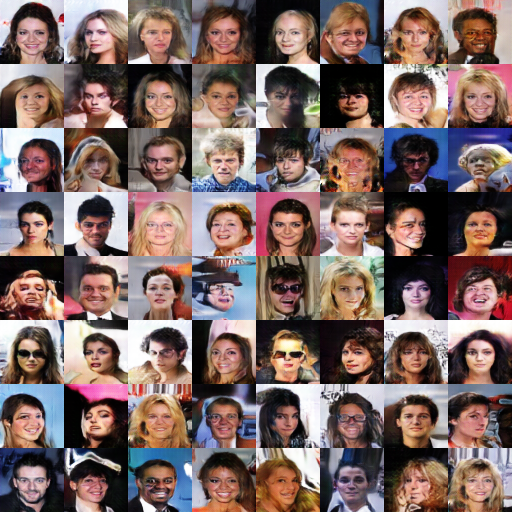
\includegraphics[width=.481\linewidth]{figures/CelebA_T=5_Sample.png}
  }%
  \hspace{8pt}%
  \subfloat[][]{%
    \label{fig:fig1-b}%
    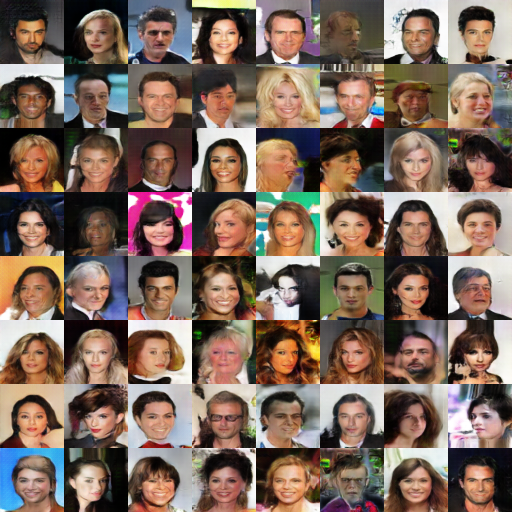
\includegraphics[width=.481\linewidth]{figures/CelebA_T=1_Sample.png}
  }\\
  \caption[Figure 1]{MIX+DCGAN vs DCGAN Samples from training on CelebA. 
    \subref{fig:fig1-a} shows samples from MIX+DCGAN with 5 Generators and 5 Discriminators; \subref{fig:fig1-b} shows samples from DCGAN.
  }
  \label{fig:ex3}%
\end{figure}

\begin{figure}[!htb]%
  \centering
  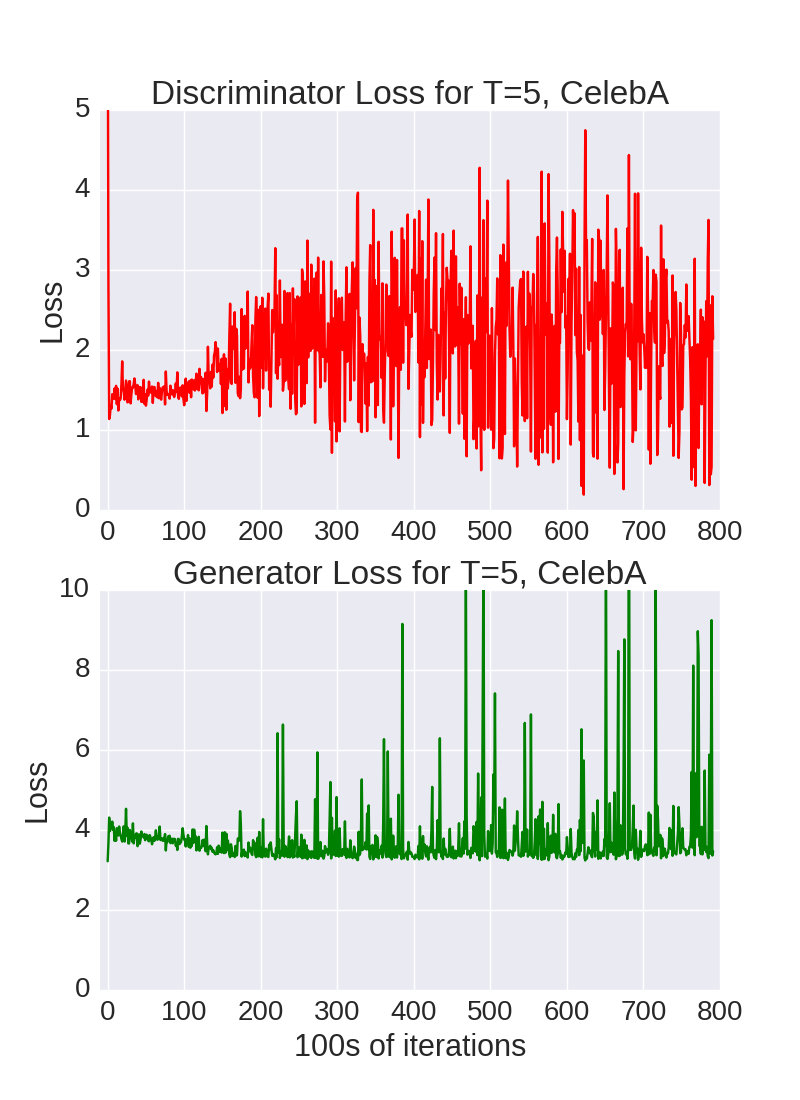
\includegraphics[width=.85\linewidth]{figures/Loss_Graph_CelebA_T=5.png}
  \caption[Figure 2]{Adversarial losses for MIX+DCGAN with 5 Generators and 5 Discriminators from training on CelebA}
  \label{fig2}
\end{figure}

\begin{figure}[!htb]%
  \centering
  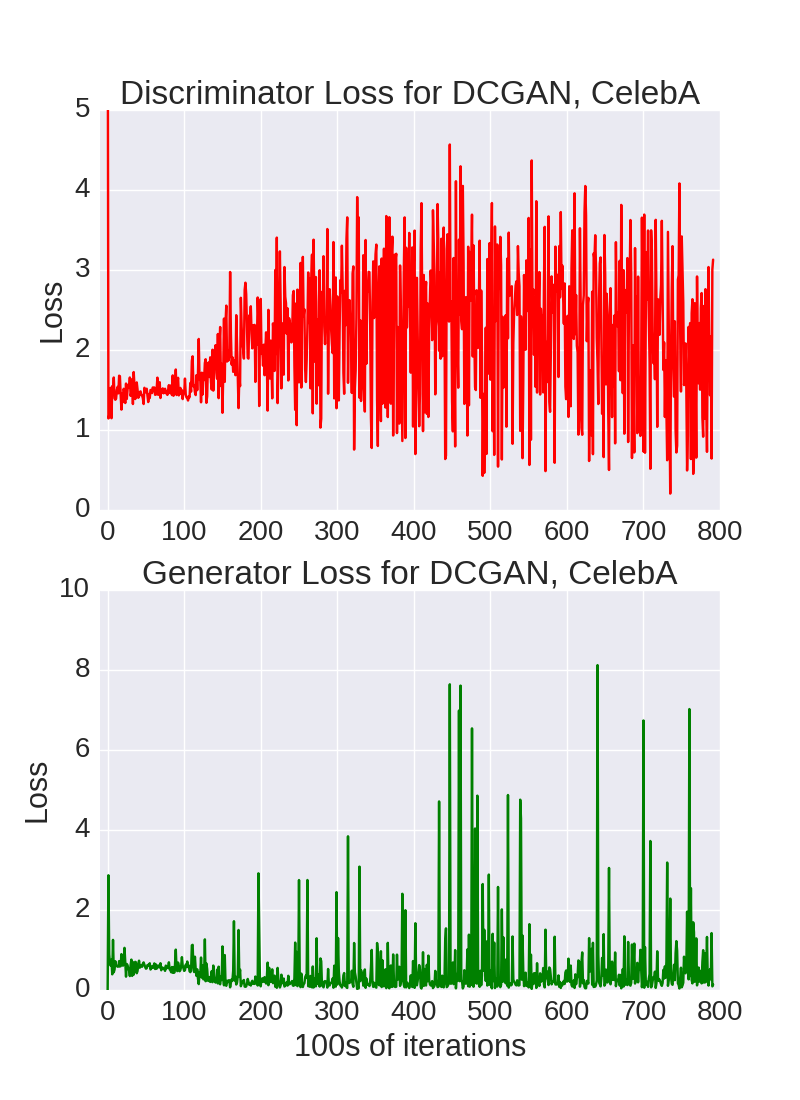
\includegraphics[width=.85\linewidth]{figures/Loss_Graph_CelebA_T=1.png}
  \caption[Figure 3]{Adversarial losses for DCGAN from training on CelebA}
  \label{fig3}
\end{figure}

\begin{figure}[!htb]%
  \centering
  \subfloat[][]{%
    \label{fig:fig4-a}%
    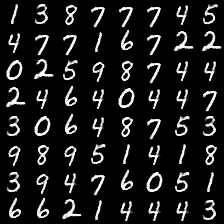
\includegraphics[width=.481\linewidth]{figures/MNIST_T=5_Sample.png}
  }%
  \hspace{8pt}%
  \subfloat[][]{%
    \label{fig:fig4-b}%
    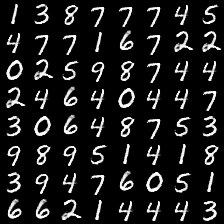
\includegraphics[width=.481\linewidth]{figures/MNIST_T=1_Sample.png}
  }\\
  \caption[Figure 4]{MIX+DCGAN vs DCGAN Samples from training on MNIST. 
    \subref{fig:fig4-a} shows samples from MIX+DCGAN with 5 Generators and 5 Discriminators; \subref{fig:fig4-b} shows samples from DCGAN.
  }
  \label{fig:ex4}%
\end{figure}

\begin{figure}[!htb]%
  \centering
  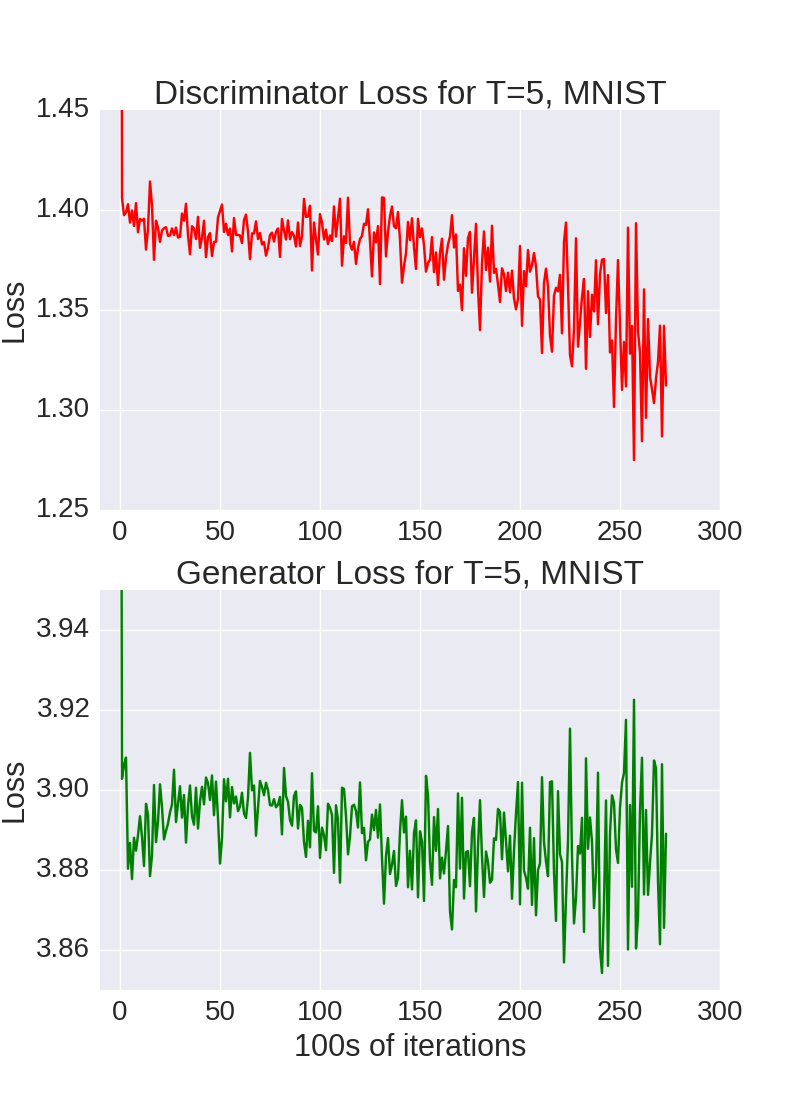
\includegraphics[width=.85\linewidth]{figures/Loss_Graph_MNIST_T=5.png}
  \caption[Figure 5]{Adversarial losses for MIX+DCGAN with 5 Generators and 5 Discriminators from training on MNIST}
  \label{fig5}
\end{figure}

\begin{figure}[!htb]%
  \centering
  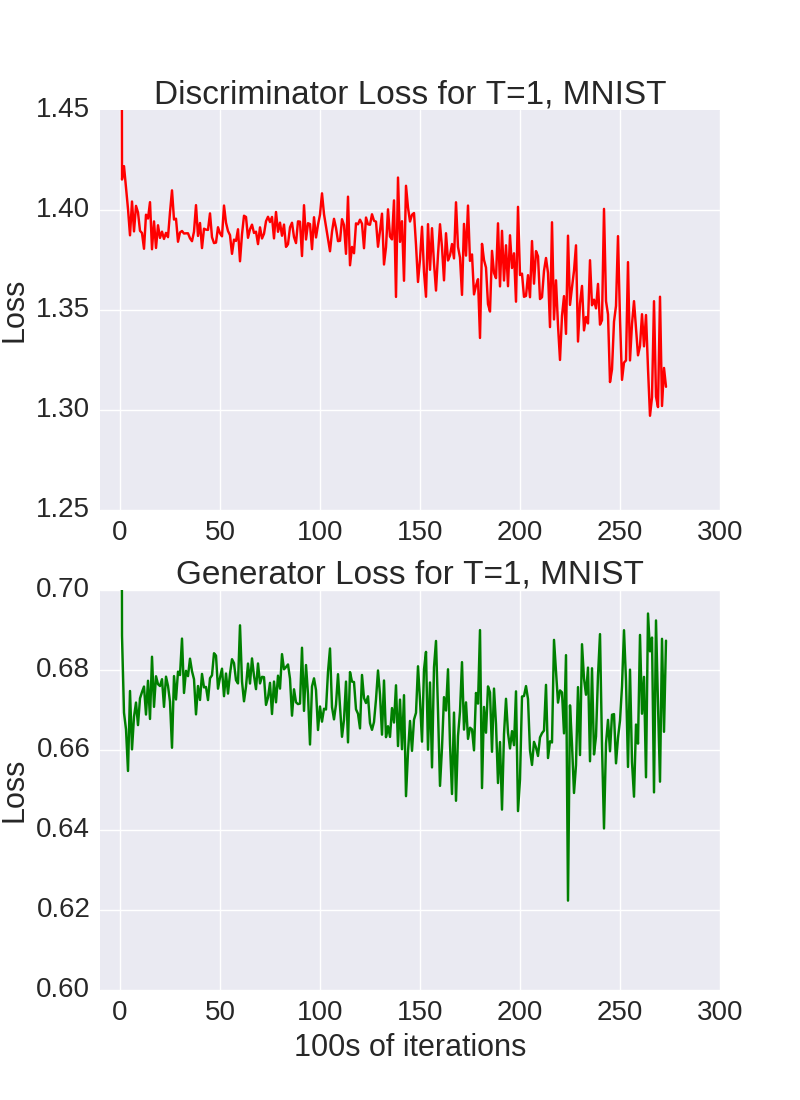
\includegraphics[width=.85\linewidth]{figures/Loss_Graph_MNIST_T=1.png}
  \caption[Figure 6]{Adversarial losses for DCGAN from training on MNIST}
  \label{fig6}
\end{figure}


\end{document}
